\documentclass[12pt]{report}
\usepackage[utf8]{inputenc}
\usepackage[russian]{babel}
%\usepackage[14pt]{extsizes}
\usepackage{listings}

% Для листинга кода:
\lstset{ %
language=python,                 % выбор языка для подсветки (здесь это С)
basicstyle=\small\sffamily, % размер и начертание шрифта для подсветки кода
numbers=left,               % где поставить нумерацию строк (слева\справа)
numberstyle=\tiny,           % размер шрифта для номеров строк
stepnumber=1,                   % размер шага между двумя номерами строк
numbersep=5pt,                % как далеко отстоят номера строк от подсвечиваемого кода
showspaces=false,            % показывать или нет пробелы специальными отступами
showstringspaces=false,      % показывать или нет пробелы в строках
showtabs=false,             % показывать или нет табуляцию в строках
frame=single,              % рисовать рамку вокруг кода
tabsize=2,                 % размер табуляции по умолчанию равен 2 пробелам
captionpos=t,              % позиция заголовка вверху [t] или внизу [b] 
breaklines=true,           % автоматически переносить строки (да\нет)
breakatwhitespace=false, % переносить строки только если есть пробел
escapeinside={\#*}{*)}   % если нужно добавить комментарии в коде
}

% Для измененных титулов глав:
\usepackage{titlesec, blindtext, color} % подключаем нужные пакеты
\definecolor{gray75}{gray}{0.75} % определяем цвет
\newcommand{\hsp}{\hspace{20pt}} % длина линии в 20pt
% titleformat определяет стиль
\titleformat{\chapter}[hang]{\Huge\bfseries}{\thechapter\hsp\textcolor{gray75}{|}\hsp}{0pt}{\Huge\bfseries}


% plot
\usepackage{pgfplots}
\usepackage{filecontents}
\usetikzlibrary{datavisualization}
\usetikzlibrary{datavisualization.formats.functions}

\begin{document}
 
%\def\chaptername{} % убирает "Глава"
\begin{titlepage}
	\centering
	{\scshape\LARGE МГТУ им. Баумана \par}
	\vspace{3cm}
	{\scshape\Large Лабораторная работа №6\par}
	\vspace{0.5cm}	
	{\scshape\Large По курсу: "Операционные системы"\par}
	\vspace{1.5cm}
	{\huge\bfseries Системный вызов open()\par}
	\vspace{2cm}
	\Large Работу выполнил: студент группы ИУ7-63Б Наместник Анастасия\par
	\vspace{0.5cm}
	\LargeПреподаватели:  Рязанова Н. Ю.\par

	\vfill
	\large \textit {Москва, 2021} \par
\end{titlepage}

%\tableofcontents

\newpage
	
Версия ядра Linux: v5.8		

Рассматриваемые структуры:


\textbf{struct filename}
\begin{lstlisting}[language=C]
struct filename {
	const char		*name;	/* pointer to actual string */
	const __user char	*uptr;	/* original userland pointer */
	int			refcnt;
	struct audit_names	*aname;
	const char		iname[];
};
\end{lstlisting}
Описание структуры находится в источнике: 

https://elixir.bootlin.com/linux/v5.8/source/include/linux/fs.h\#L2537


\textbf{struct open\_flags}
\begin{lstlisting}[language=C]
struct open_flags {
	int open_flag;
	umode_t mode;
	int acc_mode;
	int intent;
	int lookup_flags;
};
\end{lstlisting}
Описание структуры находится в источнике: 

https://elixir.bootlin.com/linux/v5.8/source/fs/internal.h\#L114


\textbf{struct open\_how}
\begin{lstlisting}[language=C]
struct open_how {
	__u64 flags;
	__u64 mode;
	__u64 resolve;
};
\end{lstlisting}
Описание структуры находится в источнике:

 https://elixir.bootlin.com/linux/v5.8/source/include/uapi/linux/openat2.h\#L19


\textbf{struct file}
\begin{lstlisting}[language=C]
struct file {
	union {
		struct llist_node	fu_llist;
		struct rcu_head 	fu_rcuhead;
	} f_u;
	struct path		f_path;
	struct inode		*f_inode;	/* cached value */
	const struct file_operations	*f_op;

	/*
	 * Protects f_ep_links, f_flags.
	 * Must not be taken from IRQ context.
	 */
	spinlock_t		f_lock;
	enum rw_hint		f_write_hint;
	atomic_long_t		f_count;
	unsigned int 		f_flags;
	fmode_t			f_mode;
	struct mutex		f_pos_lock;
	loff_t			f_pos;
	struct fown_struct	f_owner;
	const struct cred	*f_cred;
	struct file_ra_state	f_ra;

	u64			f_version;
#ifdef CONFIG_SECURITY
	void			*f_security;
#endif
	/* needed for tty driver, and maybe others */
	void			*private_data;

#ifdef CONFIG_EPOLL
	/* Used by fs/eventpoll.c to link all the hooks to this file */
	struct list_head	f_ep_links;
	struct list_head	f_tfile_llink;
#endif /* #ifdef CONFIG_EPOLL */
	struct address_space	*f_mapping;
	errseq_t		f_wb_err;
	errseq_t		f_sb_err; /* for syncfs */
} __randomize_layout
  __attribute__((aligned(4)));	/* lest something weird decides that 2 is OK */
\end{lstlisting}
Описание структуры находится в источнике: 

https://elixir.bootlin.com/linux/v5.8/source/include/linux/fs.h\#L944



\textbf{struct nameidata}
\begin{lstlisting}[language=C]
struct nameidata {
	struct path	path;
	struct qstr	last;
	struct path	root;
	struct inode	*inode; /* path.dentry.d_inode */
	unsigned int	flags;
	unsigned	seq, m_seq, r_seq;
	int		last_type;
	unsigned	depth;
	int		total_link_count;
	struct saved {
		struct path link;
		struct delayed_call done;
		const char *name;
		unsigned seq;
	} *stack, internal[EMBEDDED_LEVELS];
	struct filename	*name;
	struct nameidata *saved;
	unsigned	root_seq;
	int		dfd;
	kuid_t		dir_uid;
	umode_t		dir_mode;
} __randomize_layout;
\end{lstlisting}
Описание структуры находится в источнике: 

https://elixir.bootlin.com/linux/v5.8/source/fs/namei.c\#L502


\begin{center}
		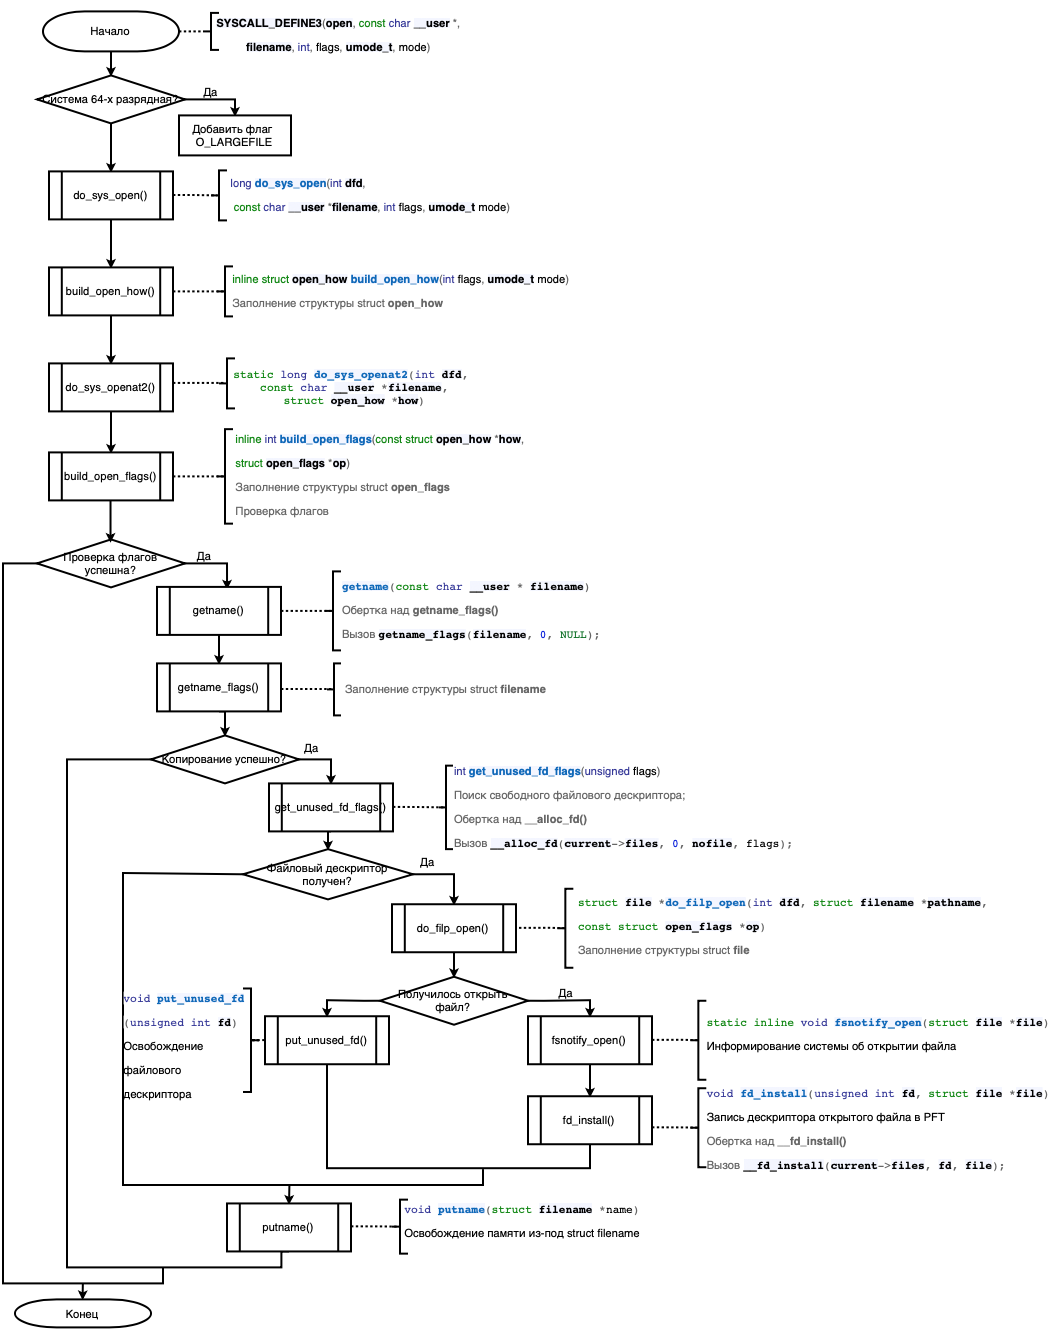
\includegraphics[scale=0.95]{pics/part1.png}
\end{center}

\begin{center}
		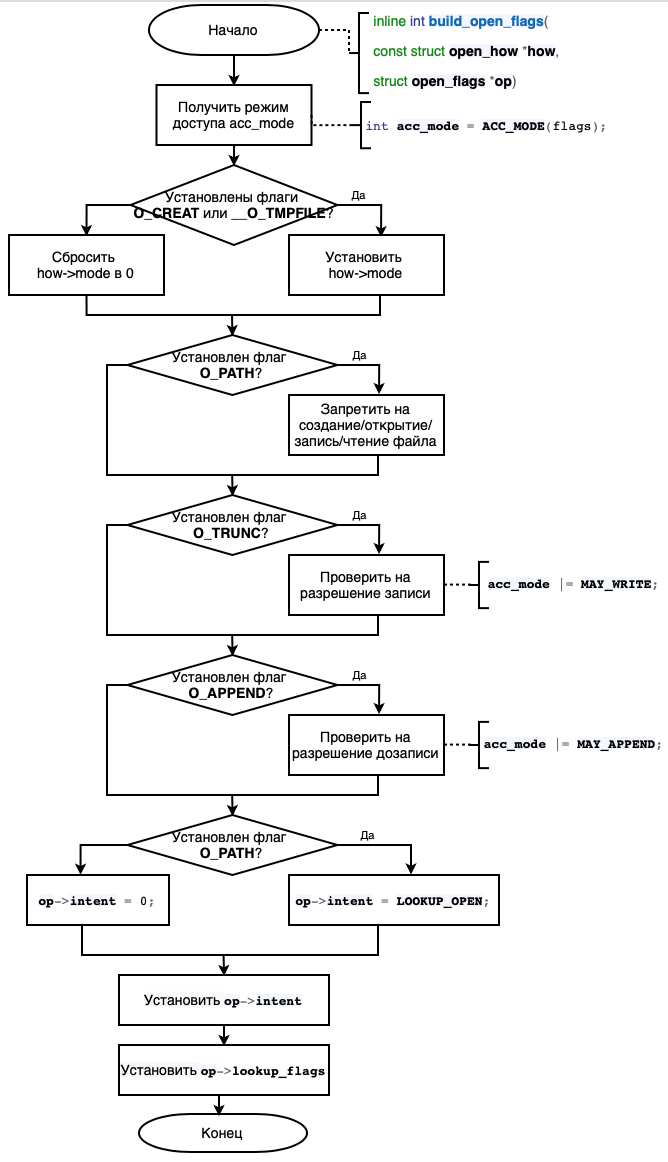
\includegraphics[scale=0.95]{pics/part2.png}
\end{center}

\begin{center}
		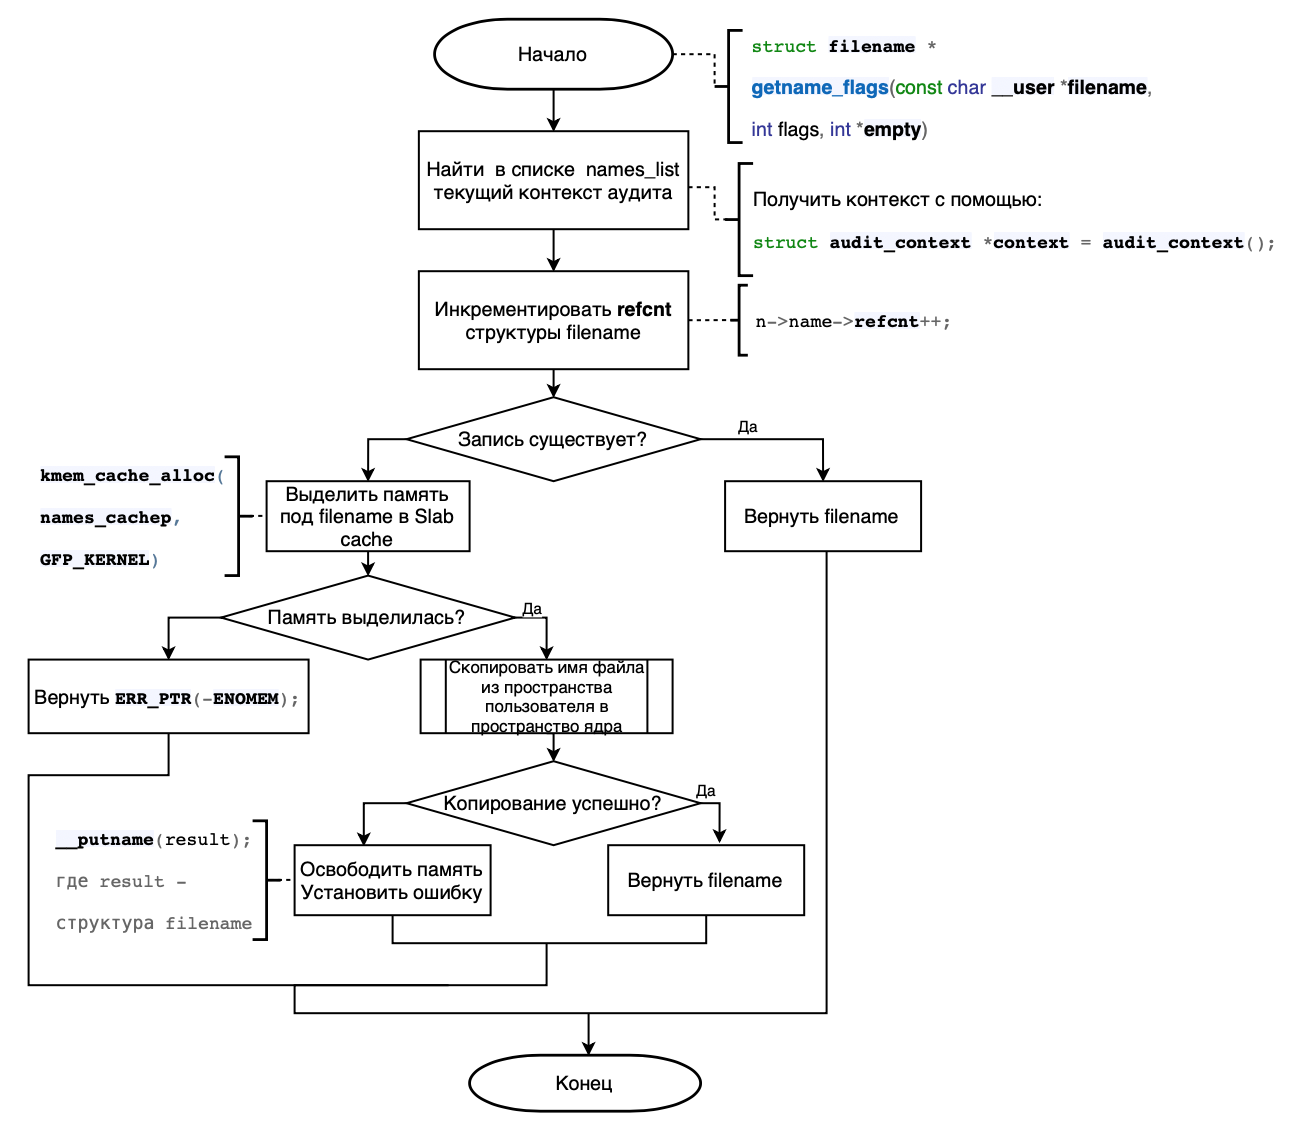
\includegraphics[scale=0.75]{pics/part3.png}
\end{center}

\begin{center}
		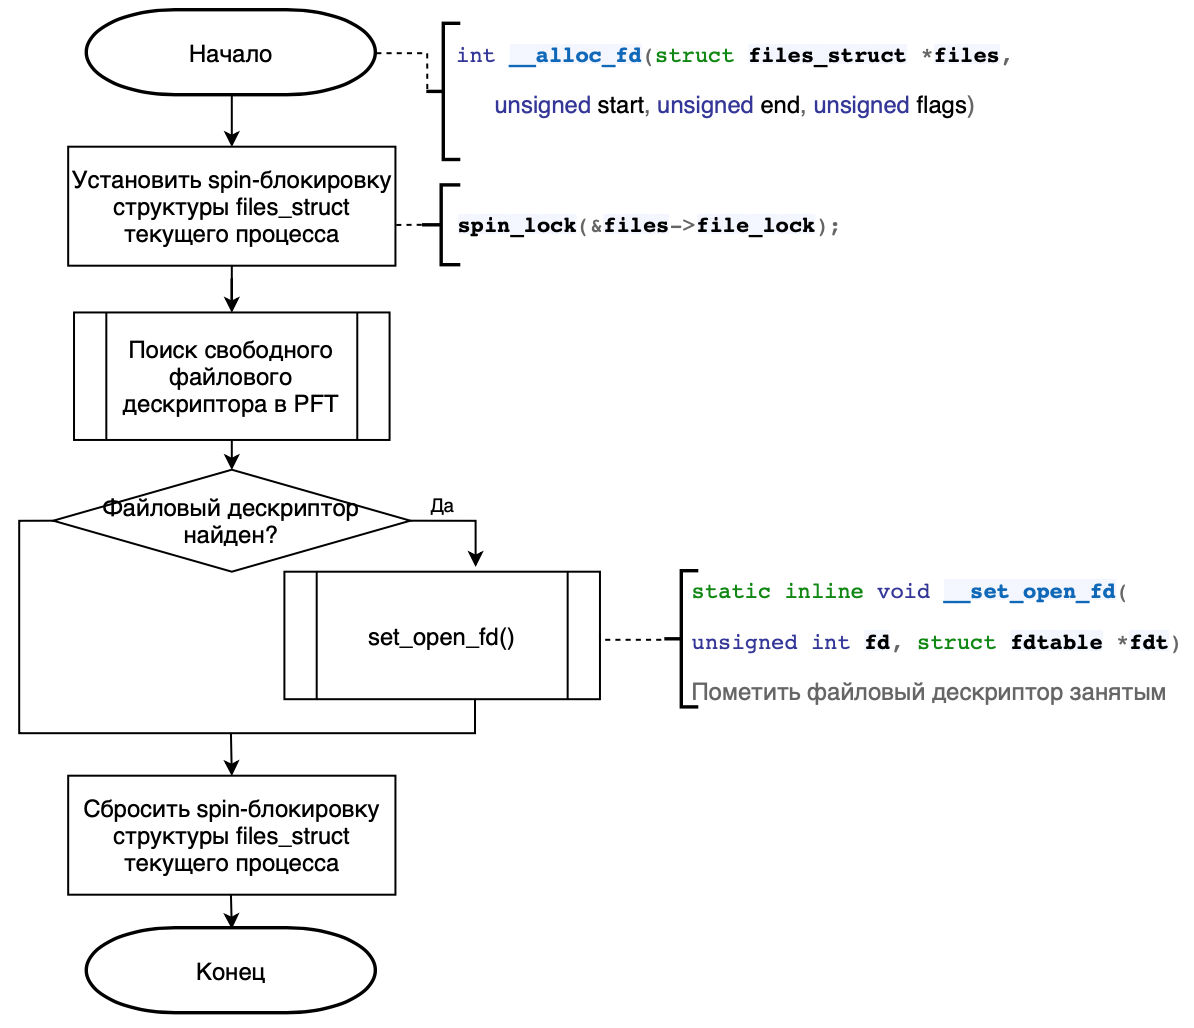
\includegraphics[scale=0.75]{pics/part4.png}
\end{center}

\begin{center}
		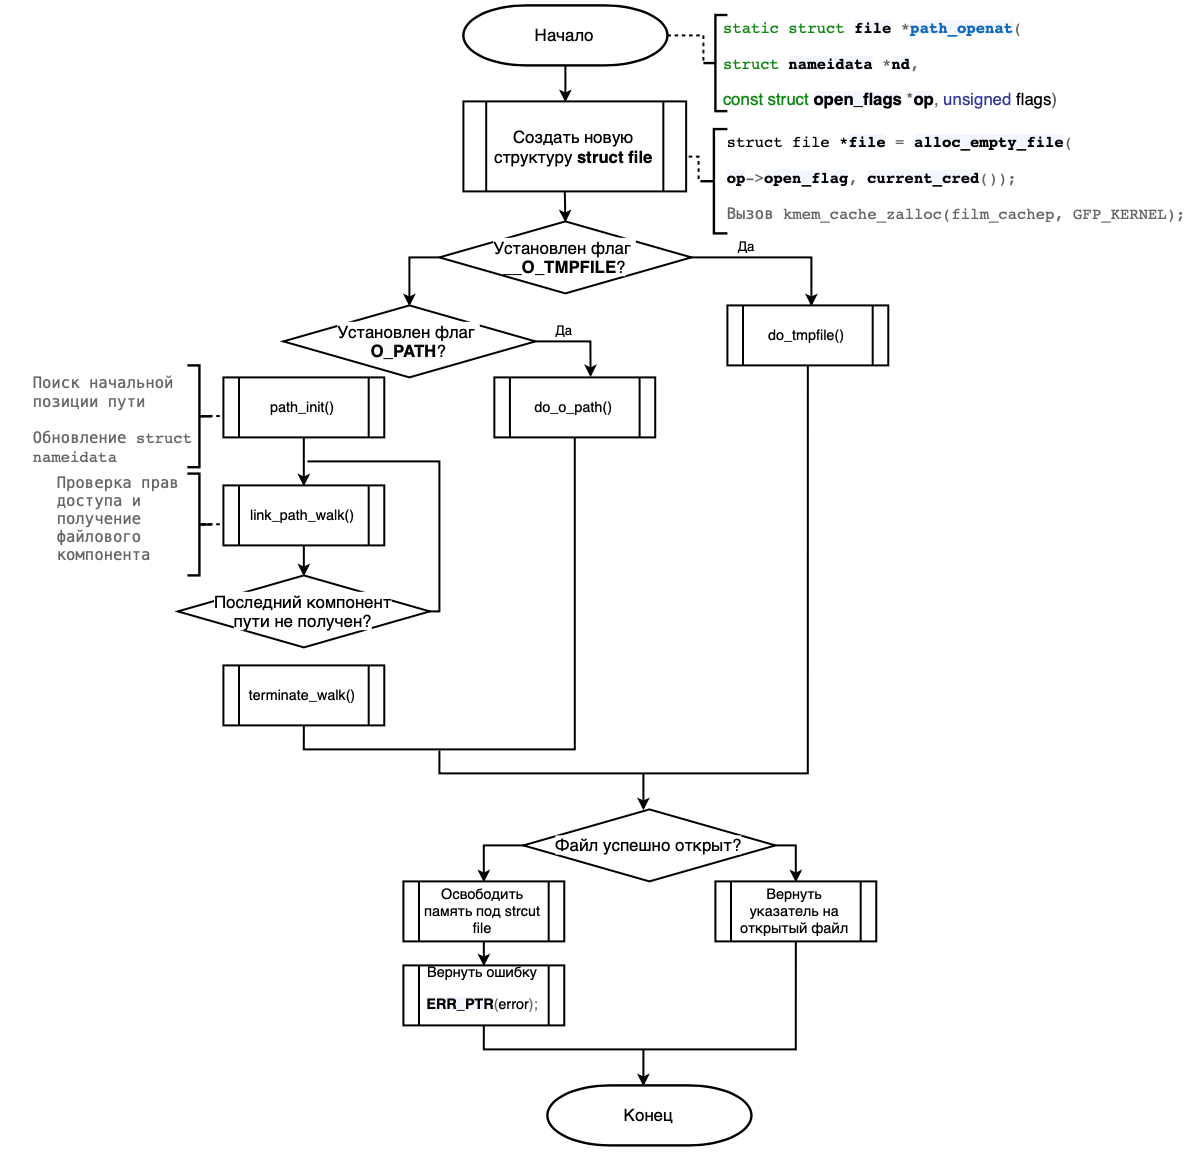
\includegraphics[scale=0.75]{pics/part5.png}
\end{center}

\begin{center}
		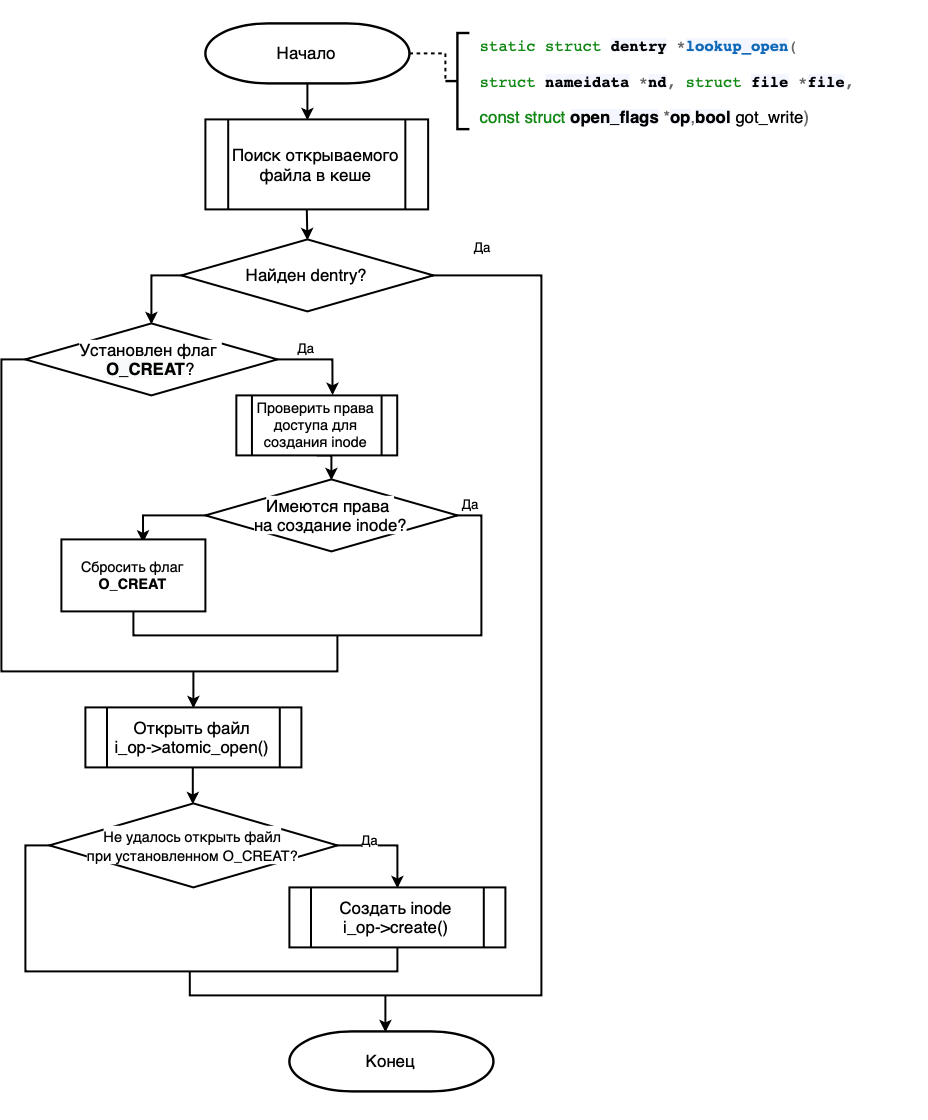
\includegraphics[scale=0.75]{pics/part6.png}
\end{center}

\section{Флаги open()}

\textbf{O\_CREAT}
(если файл не существует, то он будет создан. Владелец (идентификатор пользователя) файла устанавливается в значение эффективного идентификатора пользователя процесса. Группа (идентификатор группы) устанавливается либо в значение эффективного идентификатора группы процесса, либо в значение идентификатора группы родительского каталога (зависит от типа файловой системы, параметров подсоединения (mount) и режима родительского каталога, см. например, параметры подсоединения bsdgroups и sysvgroups файловой системы ext2.


\textbf{O\_EXCL}
(Если он используется совместно с O\_CREAT, то при наличии уже созданного файла вызов open завершится с ошибкой. В этом состоянии, при существующей символьной ссылке не обращается внимание, на что она указывает.)


\textbf{O\_NOCTTY}
(если pathname указывает на терминальное устройство, то оно не станет терминалом управления процесса, даже если процесс такового не имеет);


\textbf{O\_TRUNC}
(если файл уже существует, он является обычным файлом и режим позволяет записывать в этот файл (т.е. установлено O\_RDWR или O\_WRONLY), то его длина будет урезана до нуля. Если файл является каналом FIFO или терминальным устройством, то этот флаг игнорируется. Иначе действие флага O\_TRUNC не определено.


\textbf{O\_APPEND}
(Файл открывается в режиме добавления. Перед каждой операцией write файловый указатель будет устанавливаться в конце файла, как если бы использовался lseek); O\_APPEND (может привести к повреждению файлов в системе NFS, если несколько процессов одновременно добавляют данные в один файл. Это происходит из-за того, что NFS не поддерживает добавление в файл данных, поэтому ядро на машине-клиенте должно эмулировать эту поддержку);


\textbf{O\_NONBLOCK или O\_NDELAY}
(если возможно, то файл открывается в режиме non-blocking. Ни open, ни другие последующие операции над возвращаемым описателем файла не заставляют вызывающий процесс ждать. Для работы с каналами FIFO. Этот режим не оказывает никакого действия на не-FIFO файлы.);


\textbf{O\_SYNC}
(Файл открывается в режиме синхронного ввода-вывода. Все вызовы write для соответствующего описателя файла блокируют вызывающий процесс до тех пор, пока данные не будут физически записаны.)


\textbf{O\_NOFOLLOW}
(если pathname - это символьная ссылка, то open содержит код ошибки. Это расширение FreeBSD, которое было добавлено в Linux версии 2.1.126. Все прочие символьные ссылки в имени будут обработаны как обычно. Заголовочные файлы из glibc версии 2.0.100 (и более поздних) содержат определение этого флага; ядра версий, более ранних, чем 2.1.126, игнорируют этот флаг)


\textbf{O\_DIRECTORY}
(Если pathname не является каталогом, то open укажет на ошибку. Этот флаг используется только в Linux и был добавлен к ядру 2.1.126, чтобы избежать проблем с "отказом от обслуживания", если opendir(2) был вызван для канала FIFO или ленточного устройства. Этот флаг не следует использовать вне реализации opendir );


\textbf{O\_LARGEFILE}
(На 32-битных системах, поддерживающих файловые системы (Large), этот флаг позволяет открывать файлы, длина которых больше 31-ого бита.


\end{document}